\section{Software architecture views}
This section describes the software architecture views, it explains the subsystem decomposition, the hardware/software mapping, persistent data management and the concurrency.
\subsection{Subsystem decomposition}


\begin{figure}[h!]
  \centering
  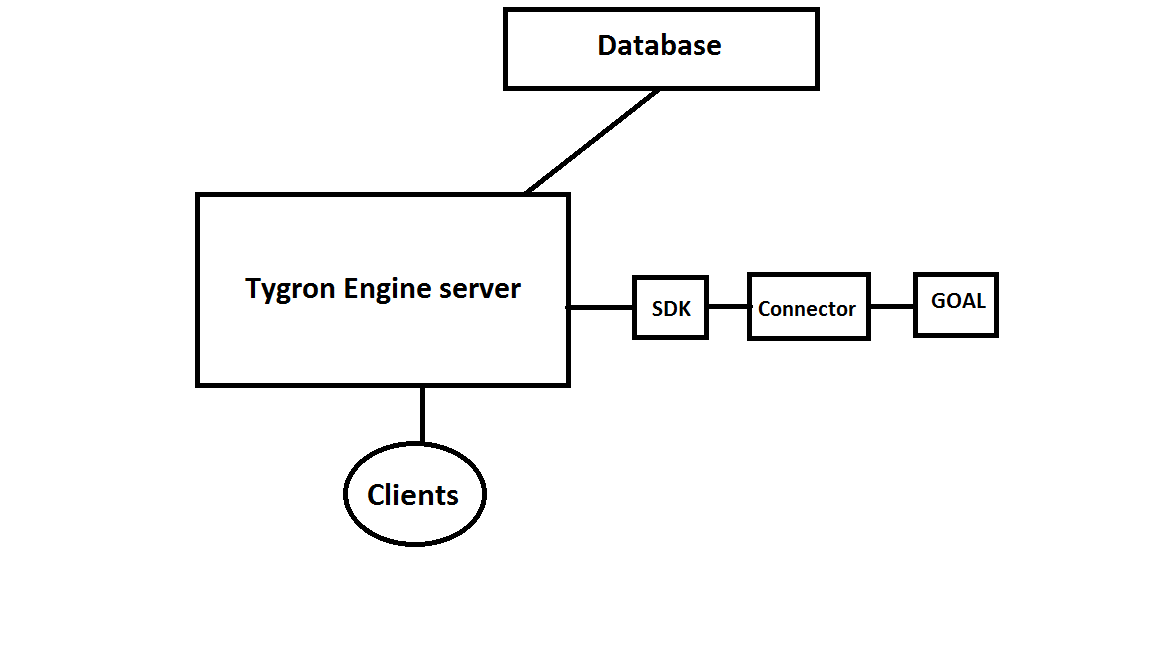
\includegraphics[scale=0.55]{Tygrondatabase3.png}
  \caption{Diagram of the Tygron Engine connected to the database and the GOAL agent.}
  \label{fig:tygron1}
\end{figure}
The architecture is divided into different subsystems. It consists of the database, Tygron engine server, several clients and several agents. In this section we will explain what each part is and does.

\begin{itemize}
	\item \textbf{The Database} \\ 
	The database in the system is used to save all kinds of data that is used to build the environment. This data contains for example the roads, buildings, rivers, etc.
	\item \textbf{The Tygron Engine Server (\textit{TES})} \\ 
	The Tygron Engine server is used to serve all the data to the correct clients and agents. The engine is an online 3D project software for urban planners, architects and engineers. It is a tool that streamlines the planning process and substantially reduces the time and costs involved in urban projects according to the Tygron website.
	\item \textbf{A Client} \\
	A client is a human interacting with the Tygron Engine Software. There can be multiple clients per \textit{TES}. The client can be a stakeholder and play the game according the strategy the stakeholder has in real life. 
	\item \textbf{The SDK} \\
	The SDK (Software Development Kit) is used to connect agents to the \textit{TES}.
	\item \textbf{An Agent} \\
	An agent is a computer controlled entity that acts like a client. There can be multiple agents per \textit{TES}. The agent can replace a client.
	\item \textbf{Connector} \\
	The connector is the link between the agent and the sdk. The agent needs the connector the run properly in the Tygron Engine. The connector generates the percepts for the agents and handles the actions that the agent performs. When an action change the environment, the agent can see the results of his action by looking at the percepts it receives from the connector.
\end{itemize}

\newpage
\subsection{Agent/Connector behaviour}
In this section some specific behaviour between the agent and the connector will be explained. The enhancements done to the connector will be explained and how they improve the development of an agent.

\subsubsection{Percepts}
In this section we'll describe some of the percepts in the connector and how our agent uses them.

	\subsubsection*{upgrade\_types percept}
		\begin{small}
			\begin{tabular}{p{2cm}p{9cm}}
				Description 	& List of upgrade types available on the map.\\
				Type 		& Send on change.\\
				Syntax 	& \verb|upgrade_types([upgrade_type(<upgradeTypeID>,|\\
						& \verb|[upgrade_pair(<sourceFunctionID>, |\\
						& \verb|<targetFunctionID>)...])...])|\\
				Parameters 	& \verb|<upgradeTypeID>|: Unique identifier for an upgrade type.\\
						& \verb|<sourceFunctionID>|: Unique identifier of the function before the upgrade.\\
						& \verb|<targetFunctionID>|:  Unique identifier of the function after the upgrade.\\
			\end{tabular}
		\end{small}
	\\To enable us to upgrade a building the specific ID of that upgrade is needed. This ID is linked to a tuple that specifies the old building and the new building after the upgrade. When we receive this percept we can select the upgrade we need and then call the action to upgrade it. By adding this our agent can upgrade a building instead of demolishing and rebuilding it.

	\subsubsection*{indicators percept}
		\begin{small}
			\begin{tabular}{p{2cm}p{9cm}}
				Description 	& List of indicators.\\
				Type 		& Send on change.\\
				Syntax 	& \verb|indicators([indicator(<indicatorID>, <currentValue>, |\\
						& \verb| <targetValue>, [zone_link(<zoneID>, <indicatorID>, |\\
						& \verb| <currentValueZone>, <targetValueZone>)...])...])|\\
				Parameters 	& \verb|<indicatorID>|: Unique identifier of the indicator.\\
						& \verb|<currentValue>|: Current value of the indicator.\\
						& \verb|<targetValue>|:  Target value of the indicator\\
						& \verb|<zoneID>|: Unique identifier of the zone.\\
						& \verb|<indicatorID>|:  Unique identifier of the indicator.\\
						& \verb|<currentValueZone>|:  Current value of the indicator for this zone.\\
						& \verb|<targetValueZone>|:  Target value of the indicator for this zone.\\
			\end{tabular}
		\end{small}
	\\The ultimate goal of the agent is to improve his score, it can do this by looking at its indicator scores and trying to improve these. To do this the agent needs to know what the score is and percept any changes. By enhancing the connector with this percept the agent is able to do this.

	\subsubsection*{indicator\_link percept}
		\begin{small}
			\begin{tabular}{p{2cm}p{9cm}}
				Description 	& Gives info about the stakeholder and weight of an indicator.\\
				Type 		& Send on change.\\
				Syntax 	& \verb|indicator_link([indicator(<indicatorID>, |\\
					 	& \verb|<stakeholderID>, <name>, <weight>...]) |\\
				Parameters 	& \verb|<indicatorID>|: Unique identifier of the indicator.\\
						& \verb|<stakeholderID>|: Unique identifier of the indicator.\\
						& \verb|<name>|:  Name of the indicator so it can be identified.\\
						& \verb|<weight>|: Weight of this indicator for the total score.\\
			\end{tabular}
		\end{small}
	\\To enable our agent to see what the weights of a certain indicator are and which indicators are his an indicator link percept has been added to the connector. This percept helps to make the indicator percept more usefull for the agent.

	\subsubsection*{buildings percept}
		\begin{small}
			\begin{tabular}{p{2cm}p{9cm}}
				Description 	& Gives info about the buildings on the map.\\
				Type 		& Send on change.\\
				Syntax 	& \verb|buildings([building(<buildingID>, <name>, |\\
					 	& \verb|<stakeholderID>, <constructionYear>, |\\
					 	& \verb|([<category>...]), <functionID>, <floors>, |\\
					 	& \verb|<multipolygon>...]) |\\
				Parameters 	& \verb|<buildingID>|: Unique identifier of the building.\\
						& \verb|<name>|: Name of the building.\\
						& \verb|<stakeholderID>|:  Unique identifier of stakeholder that owns the building.\\
						& \verb|<constructionYear>|: The construction year.\\
						& \verb|<category>|: The categories to which this building belongs.\\
						& \verb|<functionID>|: Unique identifier of the function of this building.\\
						& \verb|<floors>|: Amount of floors of this building.\\
						& \verb|<multipolygon>|: Multipolygon of the location of this building.\\
			\end{tabular}
		\end{small}
	\\The connector provides a building percept, that enables our agent to see which building he owns so that he can decide for example to destroy one of these buildings or upgrade it.

	\subsubsection*{requests percept}
		\begin{small}
			\begin{tabular}{p{2cm}p{9cm}}
				Description 	& Gives info about all the requests.\\
				Type 		& Send on change.\\
				Syntax 	& \verb|requests([request(<type>, <category>, |\\
					 	& \verb|<popupID>, <contentlinkID>, |\\
					 	& \verb|([<visibleStakeholderID>...]), ([answer(<answerID>, <description>)...]), |\\
					 	& \verb|<price>, <multipolygon>, <area>...]) |\\
				Parameters 	& \verb|<type>|: Type of the interaction.\\
						& \verb|<category>|: Category of the interaction.\\
						& \verb|<popupID>|:  Unique identifier of the request.\\
						& \verb|<contentlinkID>|: ...\\
						& \verb|<visibleStakeholderID>|: Unique ID of a stakeholder that can see this request visually in the user interface.\\
						& \verb|<answerID>|: Unique identifier of the answer.\\
						& \verb|<description>|: Answer as litteral string.\\
						& \verb|<price>|: Price of this requests if applicable.\\
						& \verb|<multipolygon>|: Multipolygon of the location of the request, usefull when for example a request is about land.\\
						& \verb|<area>|: The area of the land as in the amount of surface\\
			\end{tabular}
		\end{small}
	\\
	\\The connector provides a request percept, that enables our agent to answer to all the requests that the engine generates for our agent. For example when another stakeholder wants to buy something or asks permission.\\

\subsubsection{Add a percept}
\begin{figure}[h!]
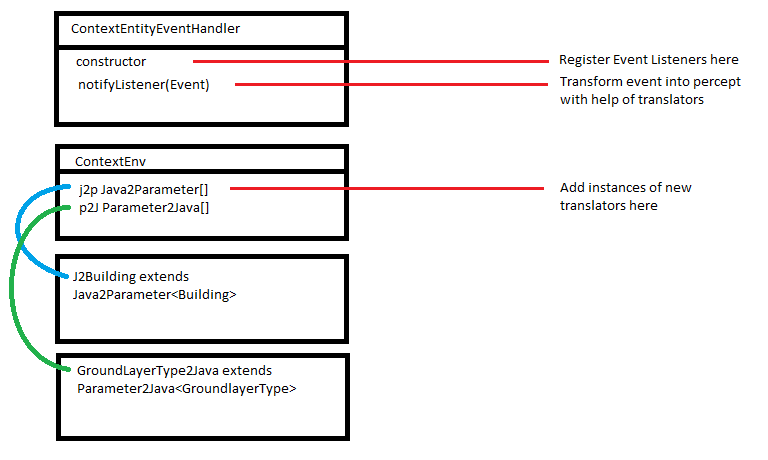
\includegraphics[width=\textwidth]{addPercept.png}
\caption{How to create a new percept}
\label{fig:addPercept}
\end{figure}

To add a new percept you will first need to create a translator, which translates java objects to parameters used in GOAL/prolog, for the object type you want to percept. Say you want to add a new buildings percept you would then create a translator for the \verb|Building| class that transforms the data you want into parameters you can use within GOAL/prolog.
After you have created this translator you want to add it to the appropriate array, \verb|Java2Parameter|, in the environment class, \verb|ContextEnv|, this will then automatically register the translator once you start a GOAL project using the environment.\\
\\
After you have done this you want to go to the \verb|ContextEntityEventHandler| class to actually start using the percept.
Here you want to register the event listener for the appropriate type, for example you would add \verb|Maplink.BUILDINGS|, then you would go to the \verb|notifyListener| method and add a case to the switch for your type, so \verb|case: BUILDINGS| for the buildings percept.
From here you can call the same method most percepts use with the appropriate type for it's argument or you can create a custom method if your percept is a little more involved.
If you use the usual method you're now done creating your new percept, but if you created a custom method make sure to add the percept to the \verb|collectedPercepts| hashmap with the event type as the key.\\
\\
After you are done creating the percept the only thing left to do is using it in a GOAL project. You can access your new percept by it's default name which it gets from the type so for \verb|Maplink.BUILDINGS| this would be |buildings|. You could also give the percept a custom name in which case you can access it with that name. Note that anyhing in GOAL/prolog that starts with a capital character will be seen as a variable so giving the percept a custom name of \verb|Buildings| wouldn't work as it won't accept a variable name as an argument in the \verb|percept| action.

\subsubsection{Actions}
\begin{figure}[h!]
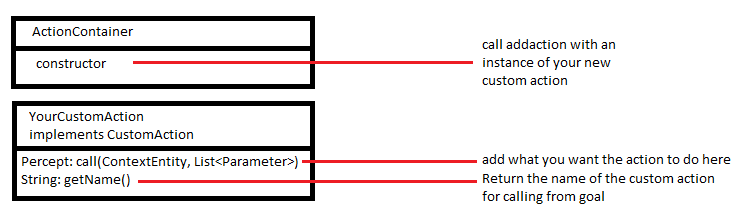
\includegraphics[width=\textwidth]{addAction.png}
\caption{How to create a custom action}
\label{fig:addAction}
\end{figure}

All available actions have been defined in the sdk, specifically in \\\verb|nl.tytech.data.engine.event.ParticipantEventType|. 
All action have a description stated in @EventParamData, this annotation also states the required parameters. 
The other annotation that all actions have is the @EventIDFields which already fills some of the parameters. 
These should then not be passed through in goal. 
Filling these in will result in the action not working at all.\\
\\
When the action you want to use requires anything but a standard string or number (float, double or integer), you will want to go ahead and add a translator for that object.
You can do this in much the same way as adding a percept.
You start of with creating a translator, but where for a percept you are converting a java object to parameters here you are translating parameters to java objects.
After you have created this translator you want to register this in the environment too, but you want to put it in a different array, \verb|Parameter2Java|, and then you are done.

\subsubsection{GOAL}

In this section we will explain how we organised our goal code.
\begin{figure}[h!]
\includegraphics[width=\textwidth]{moduleDiagram.png}
\caption{Our different modules and how they're called}
\label{fig:Modules}
\end{figure}
\\
We have devided our code in multiple modules, where the main module calls the other modules when appropiate. We illustrated this in figure 2.
The main module will never exit while there are still goals. Other modules run only once, applying the first rule that is applicable, after this they return to the main module.
For the construction of buildings we have the buildConstrucation.mod2g module that handles the construction of buildings. It is called when there is a goal to build high buildings for example. In this module, either a building is build or a goal is adopted to create land when the agent was not able to build a building.
The demolish.mod2g module is called when there is a goal to create land or an indicator goal to demolish buildings. The demolish module demolishes a building by selecting an old building that needs to be destroyed. We are currently working on a module for buying land, handling requests and upgrading buildings.
For every module there is also a test to make sure that the module is working correctly.

\subsubsection{Environment Module}

We have split of our own code into a separate, contextvh, module. 
This module is to make it easy to merge changes from other entities that work on the same base, eishub/tygron github, project.
It also helps us with testing code coverage, keeping a consistent code style and a plethora of other aspects of development since we don't have to acount for someone elses work and only need to check code we have written ourselves.


\newpage
\subsection{Hardware/software mapping}
In this section the hardware/software mapping Tygron uses will be explained, as well as the way our agent will be connected to this.

\subsubsection{Tygron}
Tygron has its own servers, from which it communicates with all other entities. For each group of users, there is a seperate server which contains the world that is used for the game and which this group of users can work on. The general Tygron server knows these other servers and will redirect the user to the particular server. So, when a customer wants to connect to Tygron, it will first connect to this general server. Also, this general server has contact with other servers which are not connected to Tygron. For example, when a customer wants to build a part of a city to play on, the general server will connect to some other servers that give information about this place, like where the buildings are and what the use of those buildings is. 

\subsubsection{Our project}

In this project there is an own server with all TU Delft students. But there is another thing that needs to be different: the way the connection is set up to that server. Since there are no humans, but agents to play the game, those agents need to connect in some way to the server. To do so, there is a connector between our instance and the server. This connector will use the goal code that is written by our group and will translate this into actions in the game. This way the agent can play the game. Figure 1 illustrates this.

\newpage
\subsection{Persistent data management}
The data management for our project envelops multiple parts. We have a part where the data for the game is stored and the data we need for running the agent. The first part is done by Tygron. When a new project is created it is stored in the Tygron database to which the clients can connect via the Tygron server. Any changes made in a session are then updated in the database, which are visible to all the other clients. Figure \ref{fig:tygron2} shows the diagram of the Tygron Engine connected to the database and the GOAL agent.

\begin{figure}[h!]
  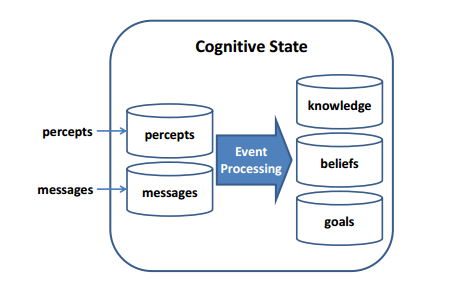
\includegraphics[width=\linewidth]{agentstate.png}
  \caption{Updating the agent's database.}
  \label{fig:agentstate1}
\end{figure}
In GOAL the data used by the agent is stored in multiple databases. The agent has a knowledge base which is the same for every environment that it might find itself in. This data is simply stored as GOAL code in the agent his GOAL files. The rest of the data that the agent uses is dynamic and its state is updated constantly according to the situation that the agent is currently in. Our agent maintains two different databases of facts. One database called the goal base consists of targets the agent wants to achieve. The other database is called the belief base and consists of facts that the agent believes are true (now). Figure \ref{fig:agentstate1} \cite{goal} shows how the databases of the agent are updated.



\newpage
\subsection{Concurrency}
Each group in the Virtual Humans for Serious Gaming context project will develop a cognitive agent, so there will be five roles and therefore multiple agents. An agent itself does not make use of concurrency, but all the agents together will run parallel and are running in one environment. When there are multiple agents running, there is concurrency. When we connect to an online server in the end, the overall system uses some networking, which also causes some concurrency. A crucial thing to find solutions for city design and development projects in a game is communication between the agents. The agents have to be able to communicate and find a solution together that fulfill the goals of the agents as much as possible.




